%!TEX root = thesis.tex

\chapter{Introduction \& Motivation}
\label{motiv:start}

Robotics in general depend heavily on \gls{hri}, which in turn is influenced and shaped by human-human interaction. %todo cite
Since speech is one of (if not) the most important form of communication between humans, it is no surprise that it is also one of the most important parts of \gls{hri}.
From a robots point of view, speech can be divided into speech synthesis and the main interest of this thesis: speech recognition.

Being able to perfectly understand the words a person spoke does not completely cover speech recognition.
See for example this video\footnote{\url{https://www.youtube.com/watch?v=iEMKZdwJPE8}} we provide or stills from it in figure \ref{pic:moti:imustgonow}.
In the video parts of a RoboCup@home Task of the RoboCup World Championship 2018 in Montreal can be seen.
In three different instances two referees are giving a robot commands, but they take turns in speaking to the robot.
The robot does not acknowledge this nor does it seem to notice.
More so: When asking for the confirmation of a specific command, it does not even seem to care that a different person gives this confirmation, or that the original referee walked away and no longer seems to care.

\begin{figure}[]
	\centering
	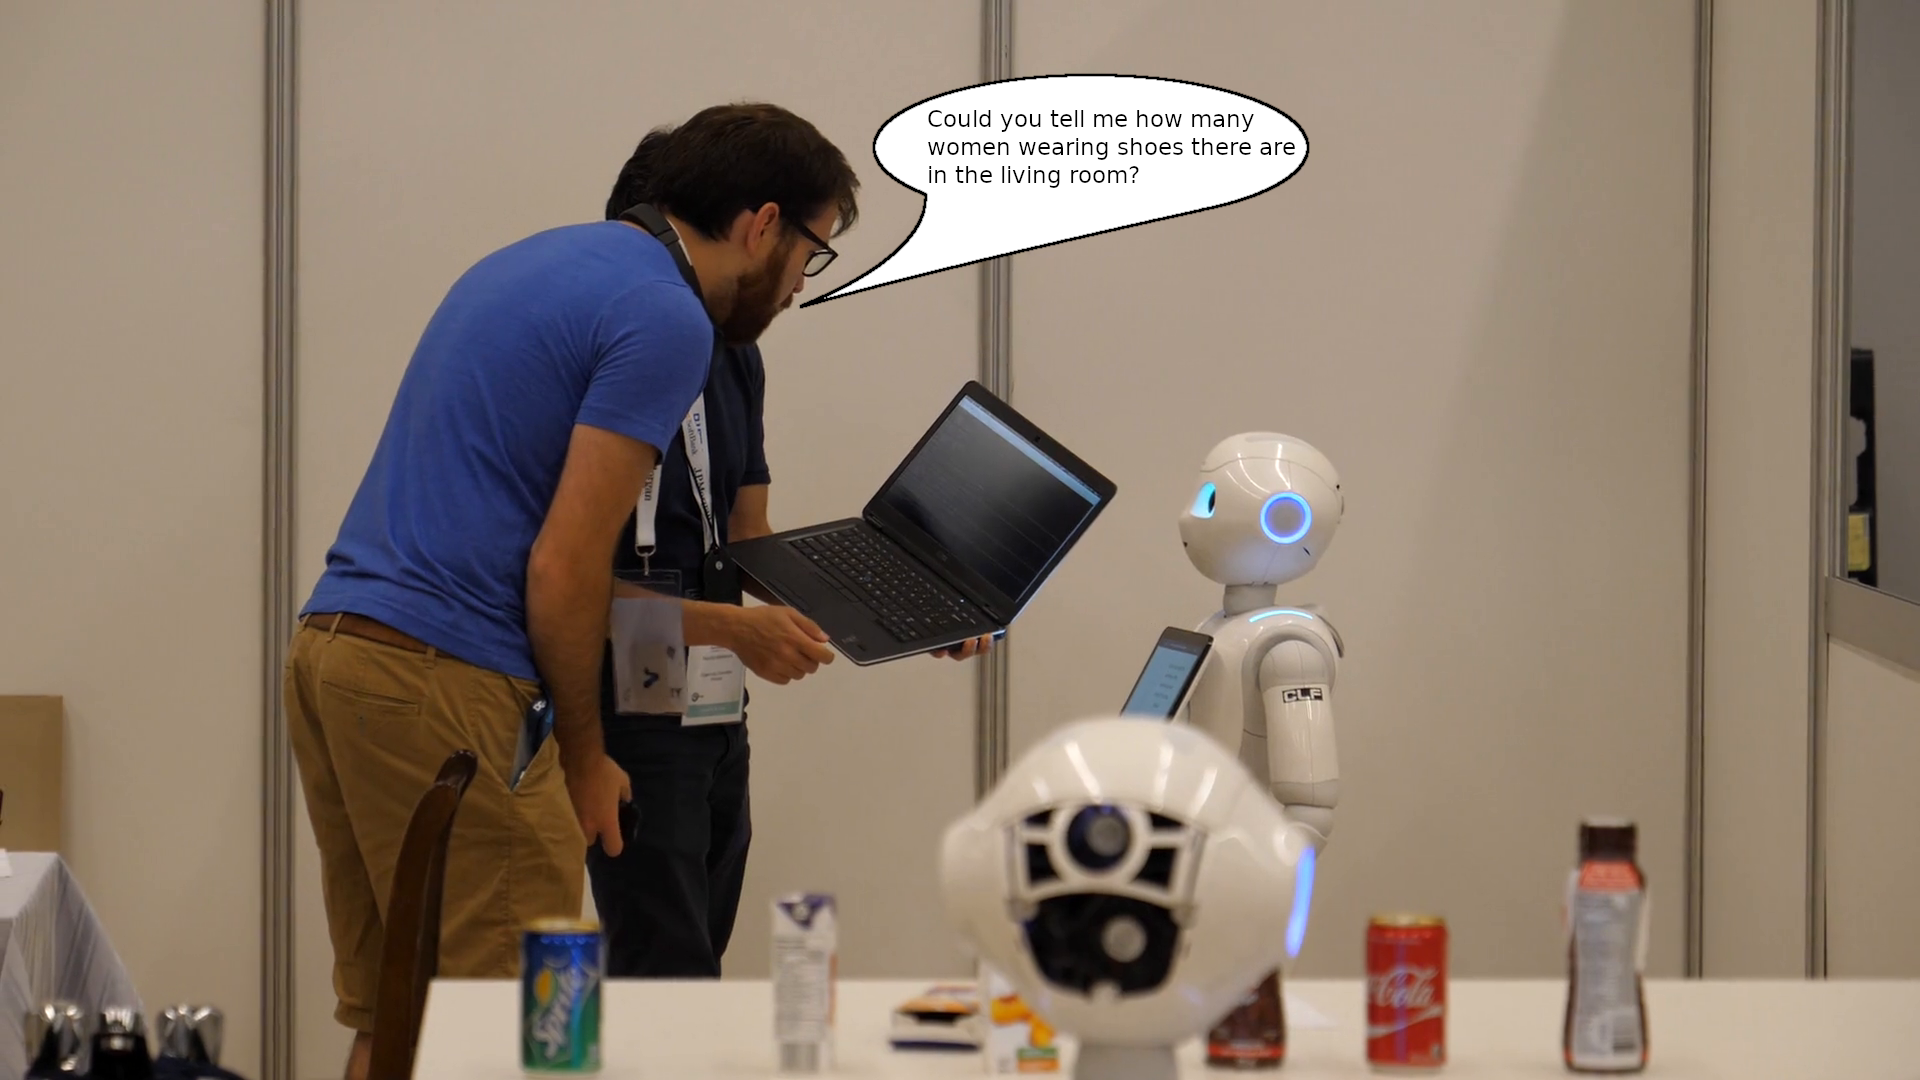
\includegraphics[width=.82\textwidth]{bilder/motivation/intro_1_edit.png}\\\vspace{3pt}
	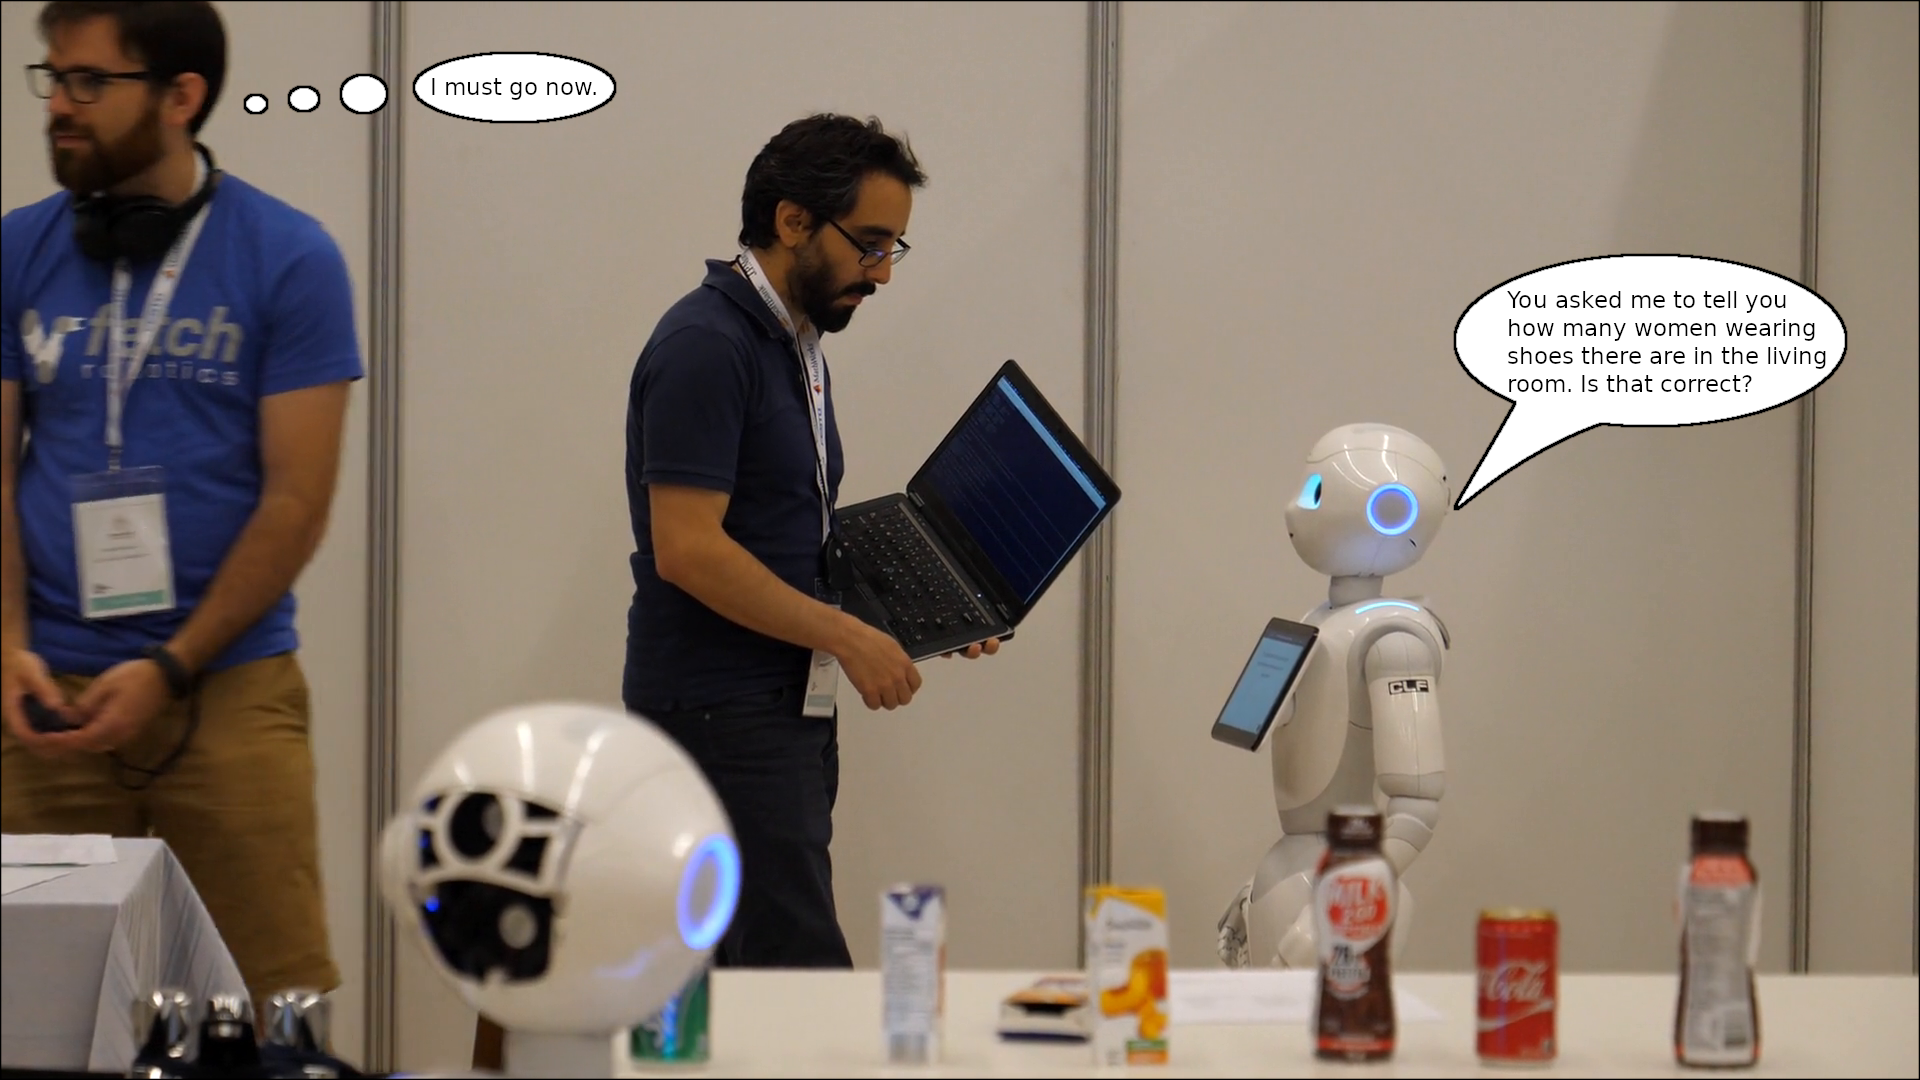
\includegraphics[width=.82\textwidth]{bilder/motivation/intro_2_edit.png}\\\vspace{3pt}
	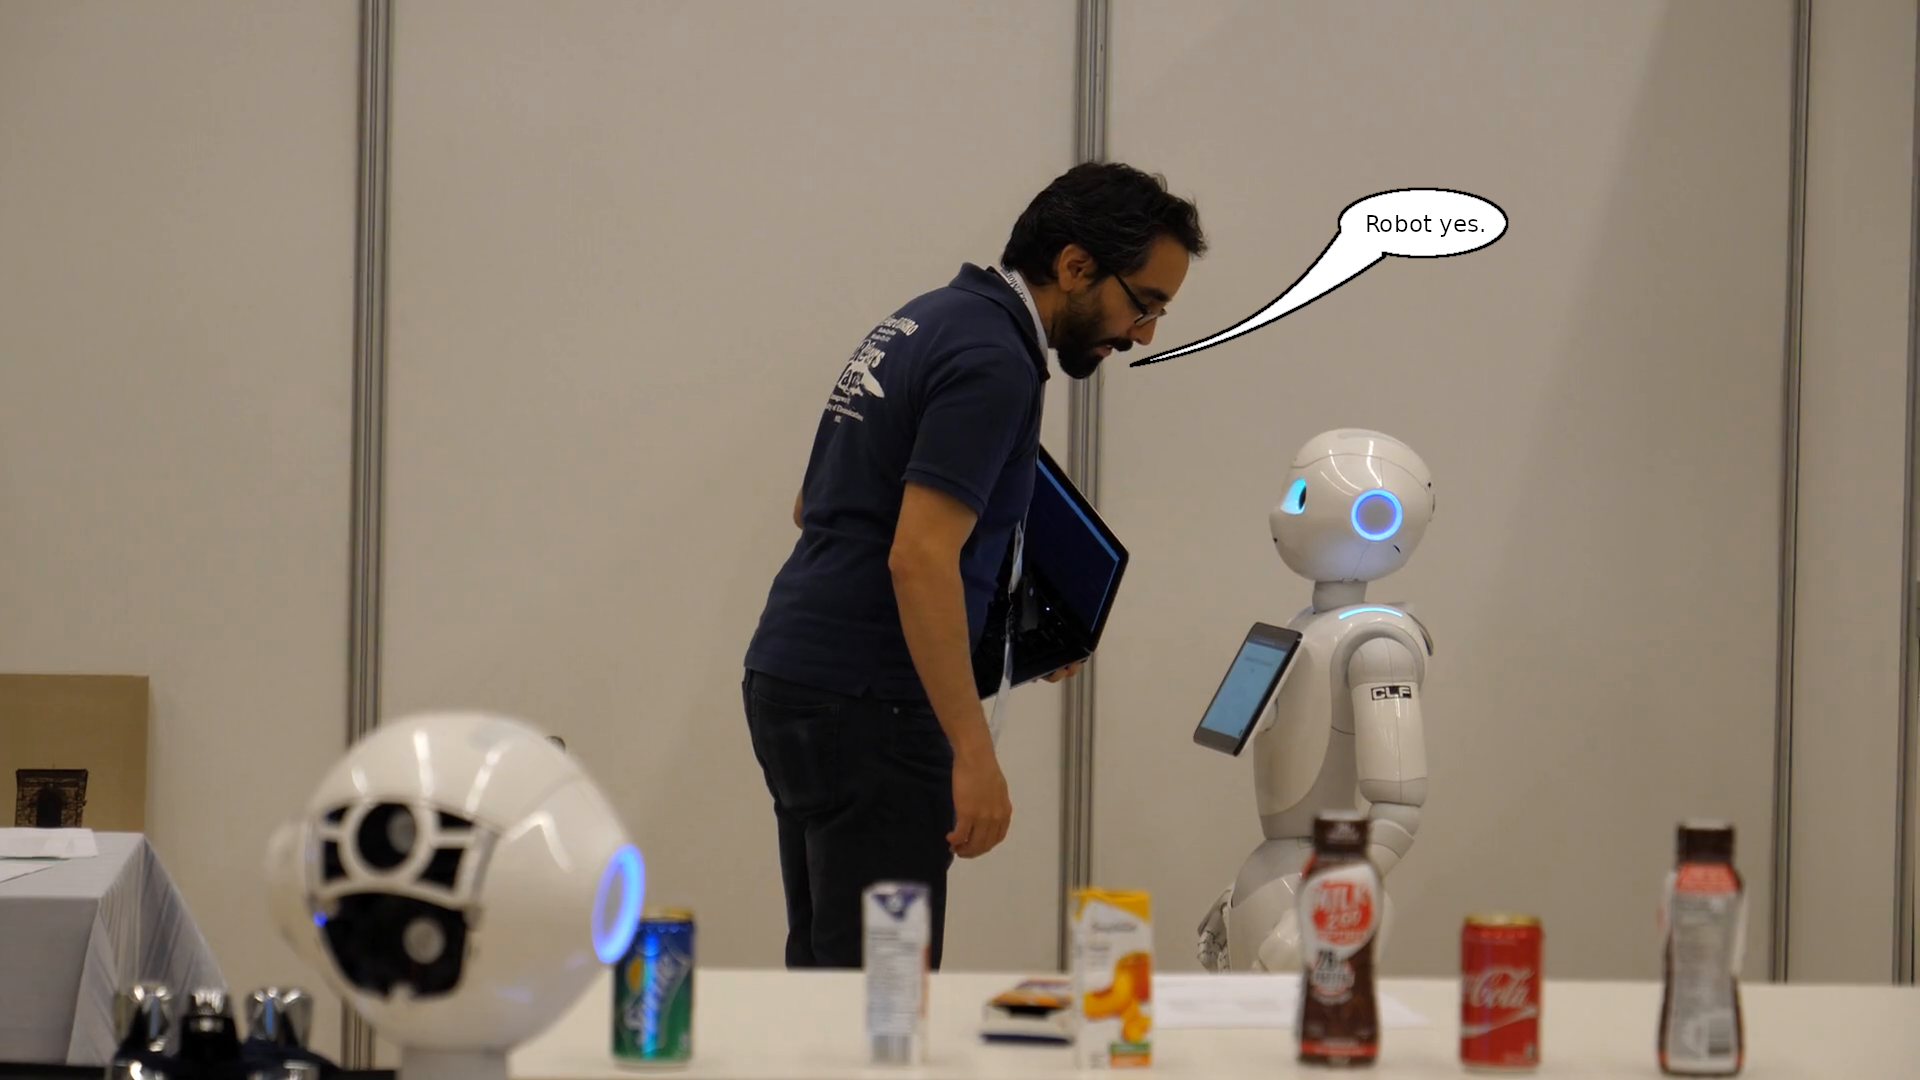
\includegraphics[width=.82\textwidth]{bilder/motivation/intro_3_edit.png}\\\vspace{3pt}
	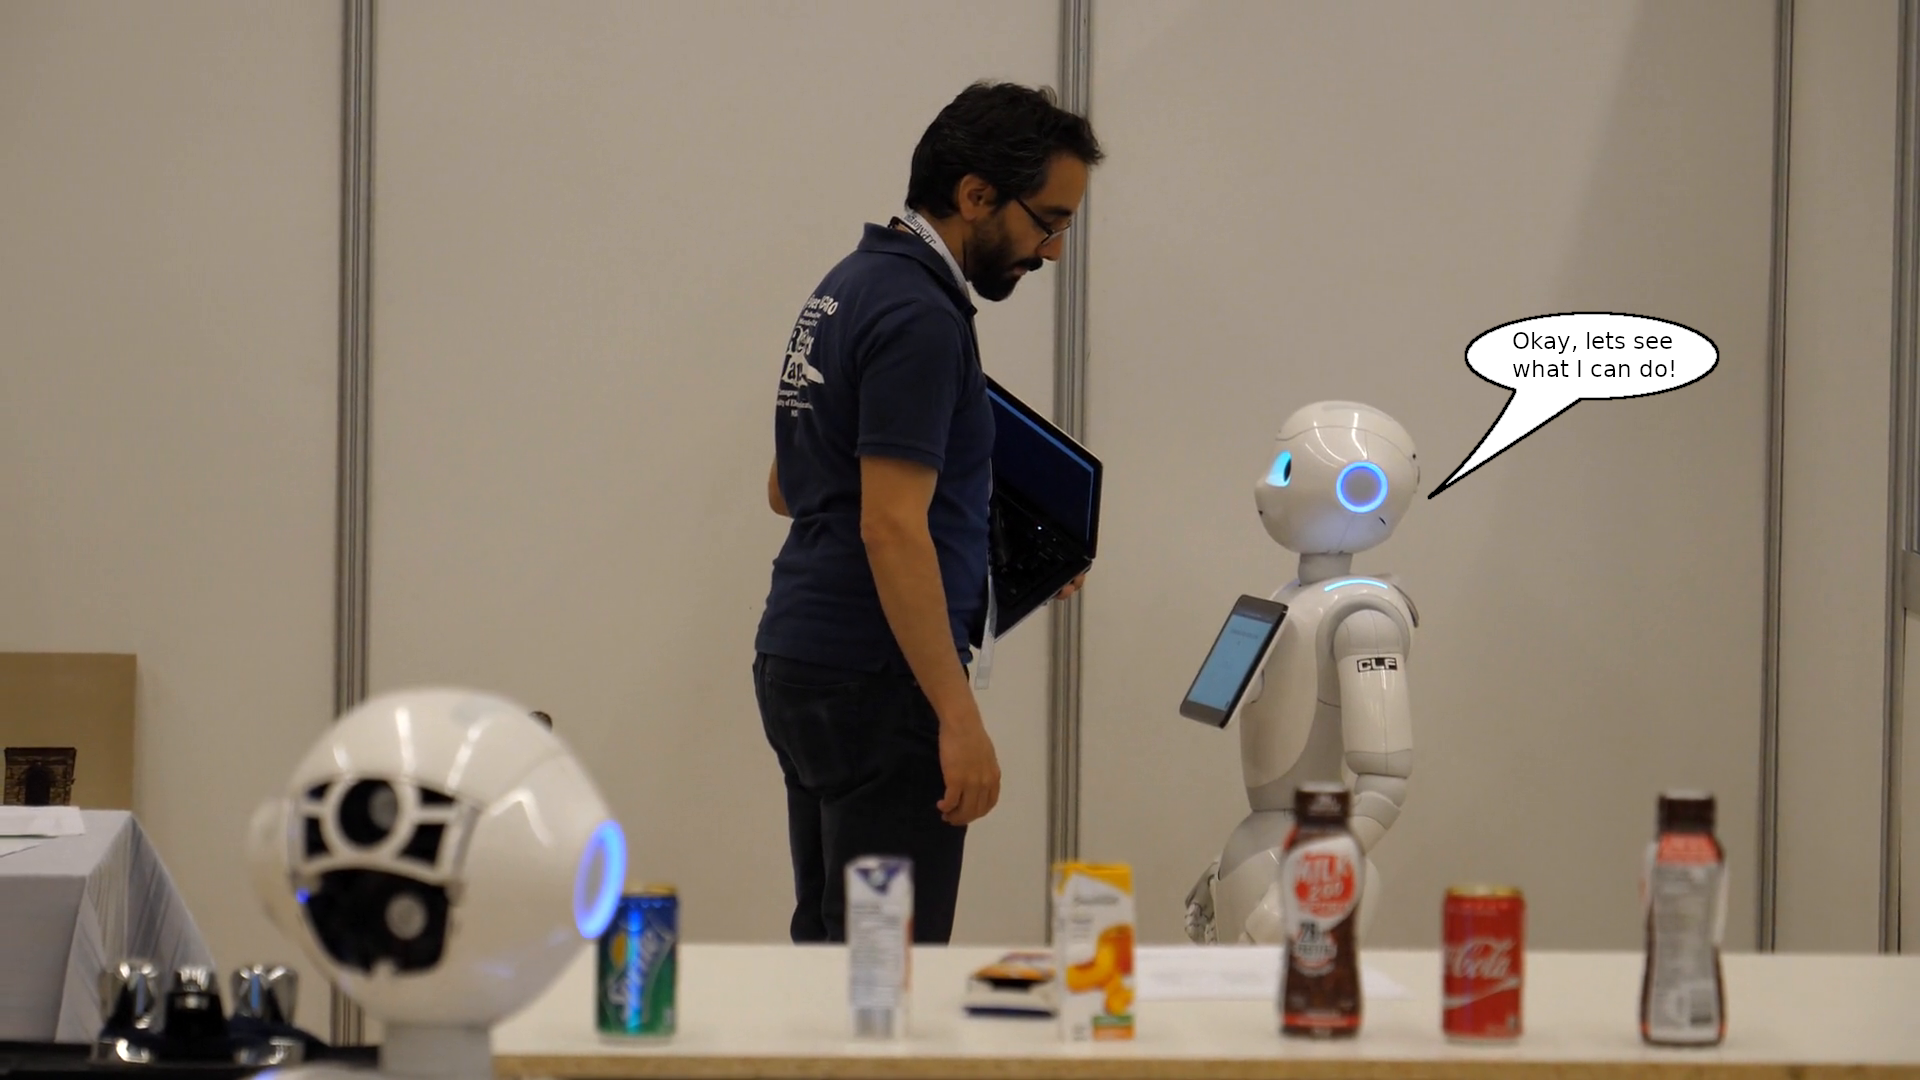
\includegraphics[width=.82\textwidth]{bilder/motivation/intro_4_edit.png}\\\vspace{3pt}
	
	\caption{Interaction between two referees and a robot in the RoboCup@home league.
		The referee in blue abandons the robot mid interaction, which does not acknowledge this at all.}
	\label{pic:moti:imustgonow}
\end{figure}

Potential security risks aside, the shown interactions appear unnatural:
The robot does not seem to really perceive the human, instead it is quite clear that it just listens for a particular combination of words.
A similar phenomenon could very publicly be observed in the near past, when Amazons Alexa ordered a variety of objects online, after hearing commands from a  TV\footnote{\url{http://archive.is/zXuJu}}.

In social robots, this behavior is not acceptable, especially since the means to at least partially solve these problems already exist.
Voice recognition technologies which can differentiate voices to a degree most people could be identified are available (todo cite voice github project).
Additionally, computer vision can be used to search for speakers, either standalone, looking for moving lips (too cite), or in combination with sound source localization (see \ref{basics:ssl}).
We will later show (see chapter \ref{related:robocup}) these to not be in use by leading robotics teams.

Of course suitable robot behaviors need to be created, to take all this information into account.
When creating these behaviors, one must take into account how these information are fed into them.
The behavior in question must either be fed a pre-combined package or be able to combine the information, e.g. a spoken utterance and a distinct, detected voice.
If the behavior handles the combination both may not be fed into the behavior at the same time, resulting in the problem to combine them.
A number of factors have to be considered when combining these informations.
Information may arrive in ratios which are not be distributed evenly.
While just a single, long speech utterance may be received, a number of voices can be detected, or several results of the same voice.
Results thus have to be combined in a manner that takes this into account.
Additionally, results will have different calculation times, based on what component created them and thus may be temporally unaligned.
This must be considered as well, creating the need to synchronize results based on their occurrence in time.

The problems just presented are clearly out of scope for robot behaviors an thus should be handled separately.
We thus declare the main goal of this thesis to be creating a framework to automatically generate these synchronized results of audio analysis solutions.

Furthermore, we can declare a number of secondary goals.
Naturally our approach to synchronize audio results shall not have a negative impact on these results.
This can be specified in two more concrete terms.
First and foremost, the accuracy of the results shall not decrease by being incorporated in our solution.
Second, synchronizing the results shall not take significantly longer to compute than not synchronizing them.
%todo elaborate

%---------------------------------- modularity secnd goal

Robotics is a field of intensive current research, and in the last years a number of leaps have been made.
These include, but are no limited to OpenPose (todo cite https://github.com/CMU-Perceptual-Computing-Lab/openpose), YOLO (todo cite https://pjreddie.com/darknet/yolo/) and DeepSpeech (todo cite https://github.com/mozilla/DeepSpeech).
Modularity and the ability to include such advances without the need to completely overhaul an existing system greatly decreases the time needed to incorporate such new technologies.
In turn, research speed can greatly benefit.
We can thus declare modularity a secondary goal, to increase the usability of the proposed framework.

%-----------------------------------

The remainder of this thesis is structured as follows:
We will first introduce a number of concepts and frameworks in chapter \ref{basics:start}.
After this we will present our solution to 
in chapter \ref{main:main}.
We will then proceed to evaluate our proposed solution in chapter \ref{eval} based on two experiments.
Lastly we will summarize our findings and point out possible future work in chapter \ref{conclusion}.

%--------------------------

%\section{old stuff}
%
%
%While other specialized fields of robotics or human robot interaction can get by just recognizing speech, social robots require more information.
%
%Humans are able to gather a plethora of information in in simple conversations which have next to nothing to do with what was actually said.
%Just by hearing a voice, one may determine a person’s emotional state, gender, or even where a person may be from, e.g. from an accent.
%A robot perceiving these information and addressing them if appropriately may lead a person interacting with the robot to feel better recognized as a person and such increase the persons acceptance of the robot.
%
%Several key features are relevant to take part in a conversation:
%The ability to match a voice/ spoken word to a (e.g. visually) perceived person, which in turn at least partially requires to recognize a voice and track the direction from where it is coming.
%Understanding whether or not a sentence or utterance was directed towards oneself.
%
%Meta information about the processes involved in speech recognition may prove useful in enabling the robot to give a user feedback on why something took longer than expected or otherwise improve interaction quality e.g. by shutting down non-essential nodes or downsampling audio data for transmission in situations where the robot is severely handicapped by low computational power or a high latency/ low throughput network respectively.
%
%What is generally known as Speech Recognition is actually comprised of several smaller subtasks, i.e. recording the raw sound, voice activity detection, and the actual speech recognition, as well as related tasks, such as sound source localization, sound filtering, beamforming, speaker recognition and addresser detection or emotion detection. %eher abstract?
%
%Speech recognition solutions tend to incorporate their basic subtasks into a single process.\todo{modularisierung eingener abschnitt?}
%This tends to entangle these subtasks to a point where code re-usability is infeasible and switching out individual subtasks is a time consuming and complex matter.
%
%\section{Synchronization of speech recognition results with related information}
%
%Speech recognition and related tasks (e.g. SSL) may take a while, especially on weaker hardware. 
%This poses a problem for systems relying on more than one of those types of data. 
%
%- synchronization between recognized speech and other information gathered by sound analysis may be tricky
%
%- to resolve synchronization issues down the line (NLP/ NLU), recognized speech should already be annotated with SSL results etc.
%
%Establishing a stable and comprehensive interface outside and inside the pipeline makes development of new components easy. 
%Evaluation of new components and benchmarking of and with existing ones can thus be greatly accelerated and encouraged.% eher auswertung?!
%
%\section{Latency}
%\todo{latency vs continuous audio signal eher in den hauptteil?}
%Latency is one of the top concerns in audio frameworks such as GStreamer and JACK (JACK Audio Connection Kit), but arguably rather unimportant in dedicated speech recognition tasks. 
%	
%Speech recognition tasks typically are bound by computationally intensive calculations, which will inherently produce a measurable latency/ delay between audio recording and recognized speech.  
%	
%For example, to recognize speech on a dynamically beamformed signal which is a typical use case with microphone arrays present on modern robots, one has to calculate sound source localization first, after which the beamformed signal can be calculated.
%If a voice activation detection is employed, it then needs to determines when a voice was picked up and and when the phrase ends, which typically takes a significant fraction of a second, thus adding to the latency. 
%	
%Because of the calculations and inherent delays, the latency introduced by the framework will almost always be rather insignificant and probably not be noticeable. 
%This holds especially true, if the point in time at which the result of the speech recognition is known can only be observed indirectly, e.g. the reaction of a robot to a spoken sentence given by a human will always be slightly delayed, just as a human typically needs a short time to react to new information, given to it verbally or otherwise.
%
%\section{Continuous Audio Signals}
%On the other hand, the possibility to lose audio frames introduces a significant problem to automated speech recognition.
%Lost audio frames result in artifacts found at the edges of neighboring frames. 
%These artifacts in turn result in unusual frequencies, which will cause problems in every step of a speech recognition pipeline which is not prepared for these to show up. 
%
%Frequency based voice activation detections and speech recognizers may not be trained with such corrupted data and produce undefined results.
%Sound source localization or beamforming solutions are particularly susceptible as they rely on several channels of audio, and if even one of them is missing, the others recorded at the same time may be unusable.
%Techniques to cope with potentially ensuing synchronization issues may also be needed to avoid undefined results.
%	
%Thus one might come to the conclusion that having a complete, discontinuity-free speech signal is more important than having a low latency.\todo{diese erkenntnis ist allerdings relativ wichtig für die motivation}
%
%
%\section{Target Audience/ Fields of Application}
%
%This work is predominantly targeted at researchers who develop new components related to speech recognition (e.g. SSL, VAD, beamforming, filtering). 
%Re-implementation of software slows down research so a framework, which allows them to easily incorporate a new algorithm/ technique into a existing pipeline of state of the art components for testing and benchmarking purposes, should improve the research speed and quality.
%
%Additional beneficiaries of this pipeline are developers who want to make use of speech recognition but do not have the resources to create their own pipeline.
%A typical user of this kind would come from the fields of robotics, which tends to be a rather interdisciplinary field, integrating more specialized fields into theirs, like speech recognition, AI, or human machine interaction.
%Giving them the opportunity to prototype and evaluate individual components and their interaction together in a standardized way.